%\documentclass[xcolor=dvipsnames]{beamer}
\documentclass[mathserif,10pt]{beamer}

\mode<presentation>
{
  \usetheme{UIUC}
} 

\newcommand{\cmt}[1]{}
\setbeamercovered{transparent=50}
\newcommand{\LIR}{{\tt LLVM IR}}
\newcommand{\MC}{{\tt Machine Code}}

\title[allvm]{allvm - Binary Decompilation}
\author{Sandeep Dasgupta}
\institute[UIUC]{University of Illinois Urbana Champaign}
\date{\today}


%if u want to show off the sections only
\setcounter{tocdepth}{1}


% If you want to come back to the subsection in outline everytime:
%\AtBeginSubsection
%{
%  \begin{frame}<beamer>{Outline}
%    \tableofcontents[currentsection,currentsubsection]
%  \end{frame}
%}

\AtBeginSection
{
  \begin{frame}<beamer>{Outline}
    \tableofcontents[currentsection,currentsubsection]
  \end{frame}
}


\begin{document}

\begin{frame}
\titlepage
\end{frame}



\section{Goal \& Motivation}
\subsection*{Research Goal}
\frame
{
  \frametitle{\subsecname}
  \begin{itemize}
    \item Research Goal
      \begin{itemize}
        \item Obtain ``richer'' LLVM IR than native machine code.
      \end{itemize}
    \item Motivation     
      \begin{itemize}
        \item Absence of source-code
        \item What-you-see-is-not-what-you-execute
        \item End-user security enforcement
        \item Platform aware optimizations
      \end{itemize}
  \end{itemize}

  \cmt{ 

    Goal involves experimental understanding of the trade-offs between
      different approaches to reconstructing LLVM IR.

    why llvm ir: We will use the LLVM Internal Representation (IR) [26] as this
      code format because the LLVM IR enables sophisticated analysis,
           optimization, and code generation for code from arbitrary languages
             at ar- bitrary points in the lifetime of software [24]. For
             example, a program in LLVM form can be optimized at traditional
             compile time, link time, install time, load time, run-time,
           “idle-time” (i.e., between runs on an end-user’s machine), or any
             combination of these.
    
    Can we obtain a richer code representation than native machine code for
    ap- plication software on an end-user’s system, in particular, one that
      makes the software amenable to sophisticated analysis, optimization and
      code generation?  
  Why needed:
  Absence of source-code: There are several circumstances where the original
source-code is not accessible. Some of the most prevalent reasons are listed
below: 
  - IP-protected software 
  - Third-party library and software components
  - Malicious executables 
  - Legacy executables 

  even if we have the source code, exectatble analysis after 
  converting it to IR is more beneficial than source code analysis.

  Source-code analysis not sufficient
    There are several scenarios where the source-code analysis is not
    sufficient.  An executable code might demonstrate differ- ent behavior from
    the original source code. This phenomenon is popularly known as
    What-you-see-is-not-what-you-execute 
    Modifications can happen to the source code during compilation
    (optimizations) or after the compilation process (bad code injection).
    These modifications can significantly alter the program behavior. Con-
    sequently, the exact behavior of any program can only be uncovered by
    analyzing the executable code.

    Moreover, several components of a typical software might be developed in
    multiple languages (Fortran, C and C++). The presence of different
    languages complicate the task of analyzing the source-code. In such
    scenarios, a consistent representation

  End-user security enforcement.: proposal pdf

  Platform aware optimizations
    Binaries compiled for wide distribution are often targeted for one
    particular ISA and are rarely optimized for a particular processor.  Binary
    tools on an end-user platform can apply custom transforma- tions to take
    advantage of platform-specific information like exact knowledge of the
    memory hierarchy or the precise version of multimedia instructions.
  
  }
}

\section{Possible Directions}
  \subsection{Decompile \MC \ $\rightarrow$ \LIR}
  \frame
  {
    \frametitle{\subsecname}
    \begin{itemize}
      \item Challenge: Quality     
      \begin{itemize}
        \item Reconstructing code and control flow - Much researched.
        \item Variable recovery
        \item Function \& ABI rules recovery
      \end{itemize}
    \end{itemize}

    \cmt{
        These methods make various trade-offs between ease of adoption, binary size,
        ease of shipping, and quality of the resulting LLVMIR, which directly
          affects the benefits that allvm provides.

          \item Diffrentiate data \& code.
          \item Indirect branch/call.
          \item Variable instruction size
          \item Position independent code (PIC) sequences
          \item Hand crafted assembly code
    }
  }


  \subsection{``Annotated'' \MC \ $\rightarrow$ \LIR}
  \frame
  {
    \frametitle{\subsecname}
    \begin{itemize}
      \item Challenge: Annotations must be ``minimal'' \& sufficient.
    \end{itemize}
  }

  \subsection{Ship \LIR}
  \frame
  {
    \frametitle{\subsecname}
    \begin{itemize}
      \item Challenges: Adoption, risks to intellectual property
    \end{itemize}
  }

\section{Decompile \MC \ $\rightarrow$ \LIR}
  \subsection{Variable \& Function parameter recovery}
  \frame
  {
    \frametitle{\subsecname}
    \begin{itemize}
      \item Benefit
        \begin{itemize}
          \item Enables many fundamental analysis (Dependence, Pointer analysis)
          \item Functional IR
        \end{itemize}
      \item State of the art
        \begin{itemize}
          \item Grammatech
            \begin{itemize}
              \item value set analysis (VSA) \& structure aggregate identification.
            \end{itemize}     
          \item Second Write 
            \begin{itemize}
              \item Heuristics for function parameter detection
              \item Scalable VSA
            \end{itemize}     
          \item TIE
            \begin{itemize}
              \item Type Recovery
            \end{itemize}     
        \end{itemize}
    \end{itemize}

  }

\section{Our Approach}
  \subsection*{Our Approach}
  \frame
  {
    \frametitle{\subsecname}
    \begin{itemize}
      \item Choose an existing decompilation framework.
      \item Experimentation with various variable and type recovery strategies
      \item Use the knowledge to infer ``minimal annotation''
    \end{itemize}

  }


\section{mcsema}
  \subsection{Choosing mcsema}
  \frame
  {
    \frametitle{\subsecname}
    \begin{itemize}
      \item Functional \LIR
      \item Separation of modules: CFG recovery and CFG $\rightarrow$ \LIR
      \item Actively supported and open sourced
    \end{itemize}

    \begin{figure}[h]
      \centering
        \scalebox{0.45}{
          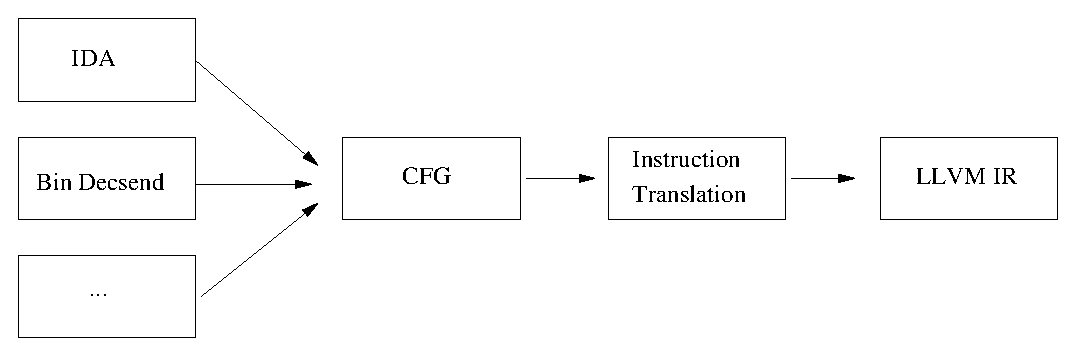
\includegraphics{Figs/1.eps}
        }
    \end{figure}
  }

  \subsection{Support \& Limitations}
  \frame
  {
    \frametitle{\subsecname}
    \begin{itemize}
      \item What Works
        \begin{itemize}
          \item Integer Instructions
          \item FPU and SSE registers
          \item Callbacks, External Call, Jump tables 
        \end{itemize}
      \item In Progress
        \begin{itemize}
          \item FPU and SSE Instructions: Not fully supported
          \item Exceptions
          \item Better Optimizations
        \end{itemize}
    \end{itemize}
  }

\section{Demo}
  \subsection{mcsema: Demo}
  \frame
  {
    \frametitle{\subsecname}
  }
\end{document}
